\documentclass{standalone}

\begin{document}

\chapter*{Appendix F - Bioinformatics Pipeline Profiling}\addcontentsline{toc}{chapter}{Appendix F - Bioinformatics Pipeline Profiling}
\markboth{Appendix F}{Profiling}

In this work many times we have talked about the performances evaluation of a scripts in terms of time performances and other system statistics.
The importance in the understanding the state of our infrastructure is essential not only for ensuring the reliability and stability of a software but also for a more efficiency use of the available resources.
In particular about what concern the memory, CPUs and diskIO management is useful to know the required amount of each step of our software to perform the better parallelization strategy.
Metrics represent the raw measurements of resource usage that are used by a software or a collection of them.
These might be low-level usage summaries provided by the operating system, or they can be higher-level types of data tied to the specific functionality or work of a component.
These kind of data could be collected and aggregated by a monitoring system like \href{https://github.com/influxdata/telegraf}{\emph{Telegraf}}\footnote{
  An automatic installation guide for Telegraf is provided in the Shut~\cite{Shut} project for any OS and also for no-root users.
}.
In general, the difference between metrics and monitoring mirrors the difference between data and information.
Monitoring takes metrics data, aggregates it, and presents it in various ways that allow humans to extract insights from the collection of individual pieces.

In this section we focused on the importance of software monitoring.
In particular we will talk about a work conducted in collaboration with INFN-CNAF of Bologna about the monitoring and the performance evaluation of a bioinformatics pipeline across various computational environments~\cite{EuroPar2018}.

In this work a previously published bioinformatics pipeline was reimplemented across various computational platforms, and the performances of its steps evaluated.
The tested environments were:
I) dedicated bioinformatics-specific server
II) low-power single node
III) HPC single node
IV) virtual machine.
The pipeline was tested on a use case of the analysis of a single patient to assess single-use performances, using the same configuration of the pipeline to be able to perform meaningful comparison and search the optimal environment/hybrid system configuration for biomedical analysis.
Performances were evaluated in terms of execution wall time, memory usage and energy consumption per patient.




\section*{GATK-LODn pipeline}\addcontentsline{toc}{section}{GATK-LODn pipeline}
\markboth{Appendix F}{GATK-LODn}

\begin{table*}
\centering
\begin{tabular}{lccccc}
\hline \rowcolor{darkgrayrow}
 & \textbf{Coverage} & \textbf{No. of} & \textbf{Read}   & \textbf{BAM file} & \textbf{NGS}\\
\rowcolor{darkgrayrow}
 &                   & \textbf{Reads}  & \textbf{Length} & \textbf{size}     & \textbf{size}\\
\hline
\textbf{Whole genome} & 37.7x & 975,000,000   & 115 & 82 GB  & 104 GB \\

\textbf{Whole genome} & 38.4x & 3,200,000,000 & 36  & 138 GB & 193 GB\\

\textbf{Exome}        & 40x   & 110,000,000   & 75  & 5.7 GB & 7.1 GB \\
\hline\\
\end{tabular}
\caption{Typical dataset size for a single patient of different types of next generation sequencing.
BAM file size refers to the size of the binary file containing the reads from the machine.}
\label{fig:wes_datasize}
\end{table*}

The pipeline used in this work, GATK-LODn, has been developed in 2016 by Do Valle et al.~\cite{DoValle2016}, and codifies a new approach aimed to Single Nucleotype Polimorphism (SNP) identification in tumors from Whole Exome Sequencing data (WES).
WES is a type of \quotes{next generation sequencing} data~\cite{Zwolak2008, Behjati2013, Shendure2008}, focused on the part of the genome that actually codifies proteins (the exome).
Albeit known that non-transcriptional parts of the genome can affect the dynamic of gene expression, the majority of cancers inducing mutations are known to be on the exome, thus WES data allow to focus the computational effort on the most interesting part of the genome.
Being the exome in human approximately 1\% of the total genome, this approach helps significantly in reducing the number of false positives detected by the pipeline.
The different sizes of next generation sequencing dataset are shown in Tab~\ref{fig:wes_datasize}.

The GATK-LODn pipeline is designed to combine results of two different SNP-calling softwares, GATK~\cite{McKenna2010} and MuTect~\cite{Cibulskis2013}.
These two softwares employ different statistical approaches for the SNP calling: GATK examines the healthy tissue and the cancerous tissue independently, and identifies the suspect SNPs by comparing them; Mutect compares healthy and cancerous tissues at the same time and has a more strict threshold of selection.
In identifying more SNPs, GATK has a higher true positive calling than Mutect, but also an higher number of false positives.
On the other end Mutect has few false positives, but often does not recognize known SNPs.
The two programs also call different set of SNPs, even when the set size is similar.
The pipeline therefore uses a combination of the two sets of chosen SNPs to select a single one, averaging the strictness of Mutect with the recognition of known variants of GATK.

The pipeline work-flow includes a series of common steps in bioinformatics analysis and in the common bioinformatics pipelines.
It includes also a sufficient representative sample of tools for the performances statistical analysis.
In this way the results extracted from the single steps analysis could be easily generalized to other standard bioinformatics pipelines.

With the increasing demand of resources from ever-growing datasets, it is not favorable to focus on single server execution, and is better to distribute the computation over cluster of less powerful nodes.
The computational pipeline also has to manage a high number of subjects, and several steps of the analyses are not trivial to be done in a highly parallel way.
Thus, the importance of system statistics management as the efficiency usage of available resources are crucial to reach a compromise between computational execution time and energy cost.
For these reasons our main focus is on the performance evaluation of a single subject without using all the available resources, as these could be more efficiently allocated to concurrently execute several subjects at the same time.
Due to the nature of the employed algorithms, not all steps can exploit the available cores in a highly efficient way: some scales sub-linearly with the number of cores, some have resource access bottleneck.
Other tools are simply not implemented with parallelism in mind, often because they are the result of the effort of small teams that prefer to focus their attention on the scientific development side rather than the computational one.

Moreover in order to obtain an optimal execution of bioinformatics pipelines, each analysis step might need very different resources.
This means that any suboptimal component of a server could act as a bottleneck, requiring bleeding edge technology if all the steps are to be performed on a single machine.
Hybrid systems could be a possible solution to these issues, but designing them requires detailed information about how to partition the different steps of the pipeline.




\section*{Computational Environments}\addcontentsline{toc}{section}{Computational Environments}
\markboth{Appendix F}{Computational Environments}

\begin{figure*}
\centering
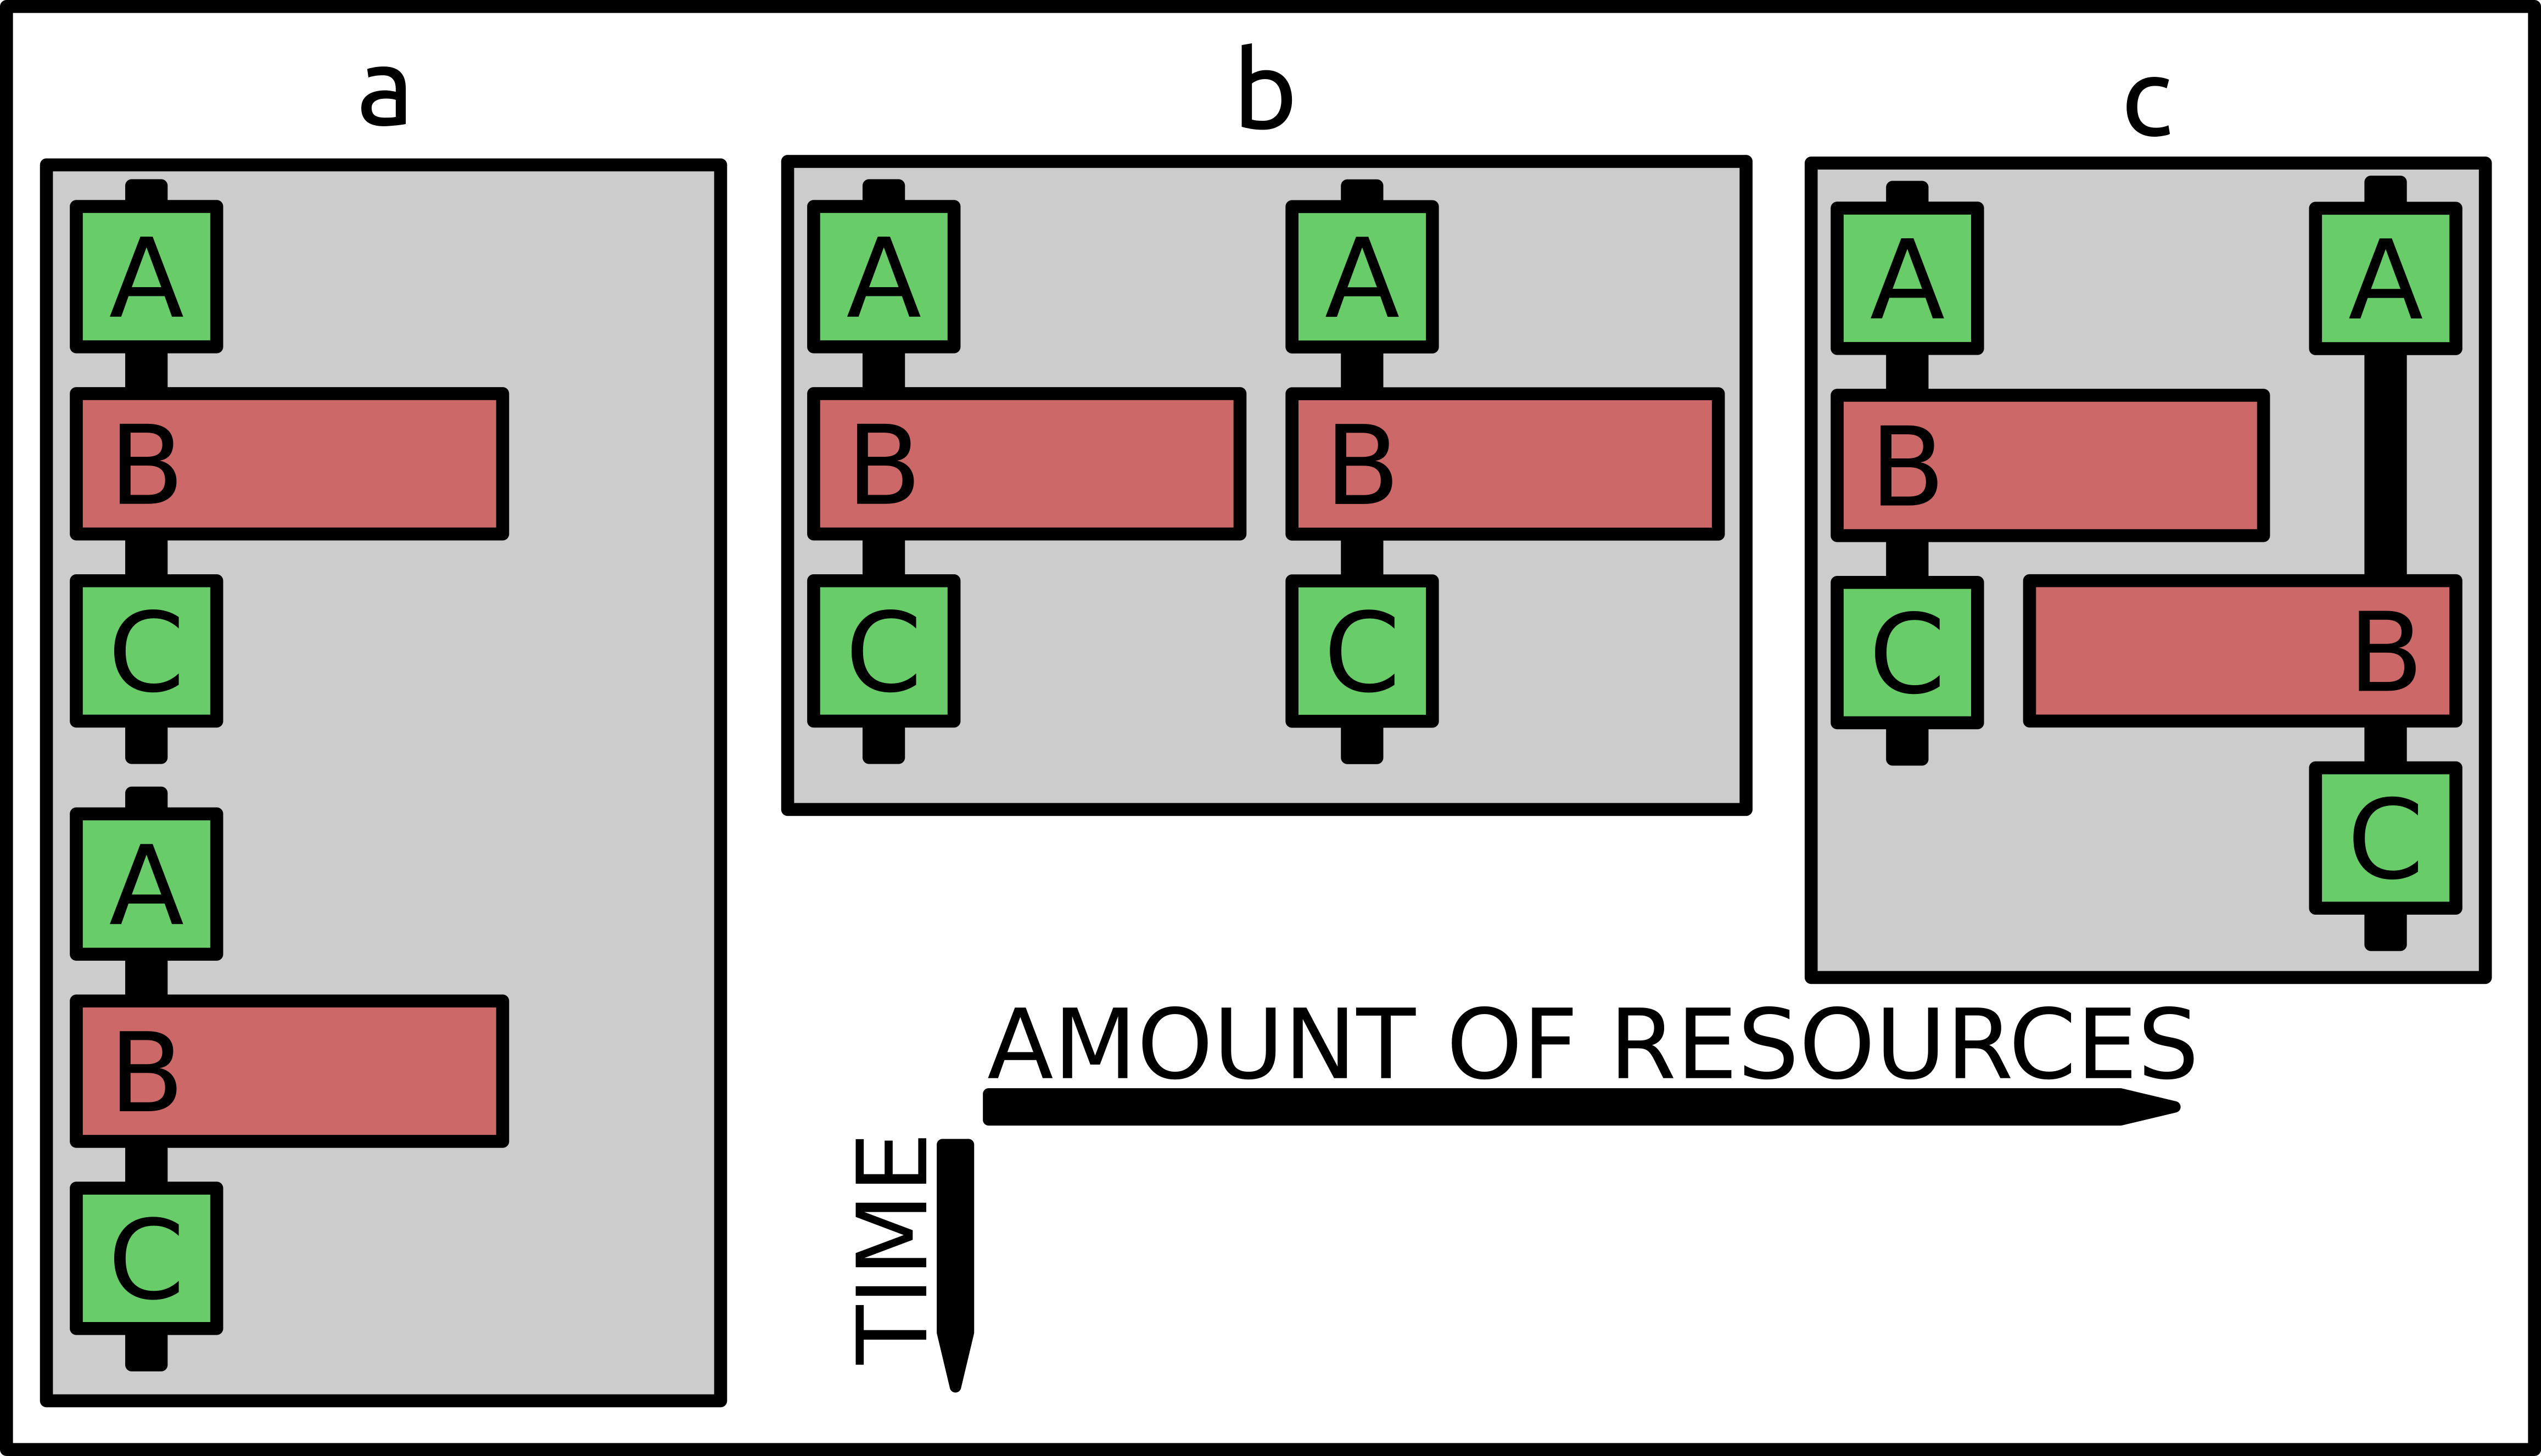
\includegraphics[width=.6\linewidth]{concurrency.png}
\caption{Examples of concurrency work-flow of two processes.
The first case ($a$) represents a simple (naive) sequential work-flow; the second ($b$) highlights a brute force parallelization; the third ($c$) is the case of a perfect match between the available resources and the requested resources.
Often brute force parallelization of pipelines done as in the image $b$ ends up overlapping the most computationally intensive steps.
Measuring the minimum viable requirements for the execution allow to better allocate resources as seen in the image $c$.}
\label{fig:wes_concurrency}
\end{figure*}

There are two main optimization strategies: the first is to improve the efficiency of a single run on a single patient and the second is to employ massive parallelization on various samples.
In both cases we have to know the necessary resources of the pipeline (and in a fine grain the resources of each step) and the optimal concurrency strategy to be applied to our work-flow (see Fig.~\ref{fig:wes_concurrency}).
In the analyses we want to highlight limits and efficiencies of the most common computational environments used in big data analytics, without any optimization strategy of the codes or systems.

We also focused on a single patient analysis, the base case study to design a possible parallelization strategy.
This is especially relevant for the multi-sample parallelization, that is the most promising of the two optimization strategies, as it does not rely on specific implementations of the softwares employed in the pipeline.

The pipeline was implemented on 5 computational environments: 1 server grade machine (Xeon E52640), 1 HPC node (Xeon E52683), 2 low power machines (Xeon D and Pentium J) and one virtual machine built on an AMD Opteron hypervisor.
The characteristics of each node are presented in Tab.~\ref{tab:node-characteristic}.

The server~-~grade node is a typical node used for bioinformatics computation, and as such features hundreds of GB of memory with multiple cores per motherboard: for these reasons we chose it as reference machine and the following results are expressed in relation to it.

The two low~-~power machines are designed to have a good cost~-~to~-~performance ratio, especially for the running cost\footnote{
  Running cost is evaluated as the energy consumption that the node requires per subject, assuming that the consumption scales linearly with the number of cores used in the individual step.
}.
These machines have been proven to be a viable solution for high performance computations~\cite{Cesini2017}.
Their low starting and running cost mean that a cluster of these machines would be more accessible for research groups looking forward to increase their computational power.

The last node is a virtual machine, designed to be operated in a cloud environment.

The monitoring tool used is \emph{Telegraf}, which is an agent written in Go for collecting, processing, aggregating, and writing metrics.
Each section of the pipeline sends messages to the \emph{Telegraf} daemon independently.

Regardless of the number of cores of each machine we restrict the number of cores used to only two to compare the statistics: this restriction certainly penalize the environment with multiple cores but with a view of maximizing the parallelizations and minimize the energy cost it is the playground to compare all the available environments.
Another restriction is applied to the chosen architectures: since available low~-~power machines provides only x86~-~architectures also the other environments are forced to work in x86 to allow the statistics comparison.

\begin{table*}
\hspace{-.75cm}
\begin{tabular}{llllll}
\hline \rowcolor{darkgrayrow}
\textbf{CLASS} & \multicolumn{2}{c}{\textbf{server grade machines}} & \multicolumn{2}{c}{\textbf{low power machines}} & \textbf{virtual machine}\\
\hline
\textbf{CPU}      & Intel Xeon  & Intel Xeon  & Intel Pentium & Intel Xeon  & AMD Opteron \\
\textbf{version}    & E5-2683v3   & E5-2640v2   & J4205   & D-1540  & 6386 SE   \\
\textbf{Microarchitecture}  & Haswell   & Ivy Bridge EP & Apollo Lake   & Broadwell   & Piledriver  \\
\textbf{Launch Date}    & Q3'14   & Q3'13   & Q4'16   & Q1'15   & Q3'12   \\
\textbf{Lithography}    & 22 nm   & 22 nm   & 14 nm   & 14 nm   & 32 nm   \\
\textbf{Cores/threads}    & 14/28   & 8/16    & 4/4     & 8/16    & 16    \\
\textbf{Base/Max Freq}    & 2.00/3.00   & 2.00/2.50   & 1.50/2.60   & 2.00/2.60   & 2.80/3.50 \\
\textbf{L2 Cache}     & 35 MB   & 20 MB   & 2 MB    & 12 MB   & 16 MB   \\
\textbf{TDP}      & 120 W   & 95 W    & 10 W    & 45 W    & 115 W   \\
\textbf{Total CPUs}     & 2     & 2     & 1     & 1     & 1   \\
\textbf{total cores/threads}  & 28/56   & 16/32   & 4/4     & 8/16    & 16    \\
\textbf{Total Memory}     & 256 GB  & 252 GB  & 8 GB    & 32 GB   & 60 GB   \\
\textbf{System power}     & 240 + 60 W  & 190 + 60 W  & 10 + 2 W  & 45 + 10 W   & 115 + 10 W  \\
\textbf{Electrical costs}   & 650 €/year  & 550 €/year  & 26 €/year   & 120 €/year  & 273€ /year  \\
\textbf{System price}   & 4000-6000 €   & 3000-5000 €   & 100-130 €   & 900-1200 €  & 2000-3000€  \\
\hline\\
\end{tabular}
\caption{Characteristics of the tested computational environments.
Electrical costs are estimated as 0.25~€/kWh; CPU frequencies are reported in GHz; TDP: Thermal Design Power, an estimation indicator of maximum amount of heat generated by a computer chip when a \quotes{real application} runs.}
\label{tab:node-characteristic}
\end{table*}



\section*{Pipeline steps}\addcontentsline{toc}{section}{Pipeline steps}
\markboth{Appendix F}{Pipeline steps}

The pipeline steps that have been examined are a subset of all the possible steps: we only focus on those whose computational requirements are higher and thus require the most computational power.
These steps are:

\begin{enumerate}

\item\textbf{mapping:} takes all the reads of the subjects and maps them on the reference genome;

\item\textbf{sort:} sorts the sequences based on the alignment, to improve the reconstruction steps;

\item\textbf{markduplicates:} checks for read duplicates (that could be imperfections in the experimental procedures and would skew the results);

\item\textbf{buildbamindex:} indexes the dataset for faster sorting;

\item\textbf{indexrealigner:} realigns the created data index to the reference genome;

\item\textbf{BQSR:} base quality score recalibration of the reads, to improve SNPs detection;

\item\textbf{haplotypecaller:} determines the SNPs of the subject;

\item\textbf{hardfilter:} removes the least significant SNPs.

\end{enumerate}

The following statistics were evaluated:

\begin{enumerate}

\item\textbf{memory per function:} estimate percentage of the total memory available to the node used for each individual step of the pipeline;

\item\textbf{energy consumption:} estimated as the time taken by the step, multiplied by the number of cores used in the step and the power consumption per core (TDP divided by the available cores). As mentioned before this normalization unavoidably penalize the multi-core machines but give us a term of comparison between the different environment;

\item\textbf{elapsed time:} wall time of each step.

\end{enumerate}

The pipeline was tested on the patient data from the 1000 genome project with access code NA12878, sample SRR1611178.
It is referred as a Gold Standard reference dataset~\cite{Zook2014}.
It is generated with an Illumina HiSeq2000 platform, SeqCap EZ Human Exome Lib v3.0 library and have a 80x coverage.
As Gold Standard reference it is commonly used as benchmark of new algorithm and for our purpose can be used as valid prototype of genome.


\section*{Results}\addcontentsline{toc}{section}{Results}
\markboth{Appendix F}{Results}

Memory occupation is one of the major drawbacks of the bioinformatics pipelines, and one of the greater limits to the possibility of parallel computation of multiple subjects at the same time.
As it can be seen in Fig.~\ref{fig:memory-per-step}, the memory occupation is comprised between 10\% and 30\% on all the nodes.
This is due to the default behavior of the GATK libraries to reserve a fixed percentage of the total memory of the node.
The authors could not find any solution to prevent this behavior from happening.
As it can be noticed, in the node with the greatest amount of total memory (both Xeon E5 and the virtual machine) the requested memory is approximately stable, as is always sufficient for the required task.
The memory allocation is less stable in the nodes with a limited memory (Xeon D and Pentium J), as GATK might requires more memory than what initially allocated to perform the calculation.
The exception to this behavior is the \quotes{mapping} step, that uses a fixed amount of memory independently from the available one (between 5 and 7 GB).
This is due to the necessity of loading the whole human reference genome (version hg19GRCh37) to align each individual read to it.
All the other steps do not require the human reference genome but can work on the individual reads, allowing greater flexibility in memory allocation.

As can be seen in Fig.~\ref{fig:performance-per-step} and Fig.~\ref{fig:energy-per-step}, this increase of memory consumption does not correspond to a proportional improvement of the time elapsed in the computation.

The elapsed time for each step and for the whole pipeline can be seen in Fig.~\ref{fig:performance-per-step}.
It can be seen that there is a non consistent trend in the behavior of the different environments.
Aside from the most extreme low power machine, the pentium J, the elapsed times are on average higher for the low power and slightly higher for the cloud node, but the time for the individual rule can vary.
In the sorting step, Pentium J is 20 times slower than the reference.
This is probably due to the limited cache and memory size of the pentium J, that are both important factors determining the execution time of a sorting algorithm and are both at least four to six times smaller than the other machines.
The HPC machine, the Xeon E52683, is consistently faster than the reference node.

The energy consumption per step can be seen in Fig.~\ref{fig:energy-per-step}.
The low power machines are consistently less than half the baseline consumption.
Even considering the peak of consumption due to the long time required to perform the sorting, the most efficient low power machine, the pentium J, consumes 40\% of the reference, and the Xeon D consumes 60\% of the reference.
The HPC machine, the Xeon E52683, have consumption close to the low power nodes, balancing out the higher energy consumption with a faster execution speed.
The virtual machine has the highest consumption despite the fact that the execution time of the whole pipeline is comparable to the reference due to the high TDP compared to its execution time.

\begin{figure*}[t!]
\centering
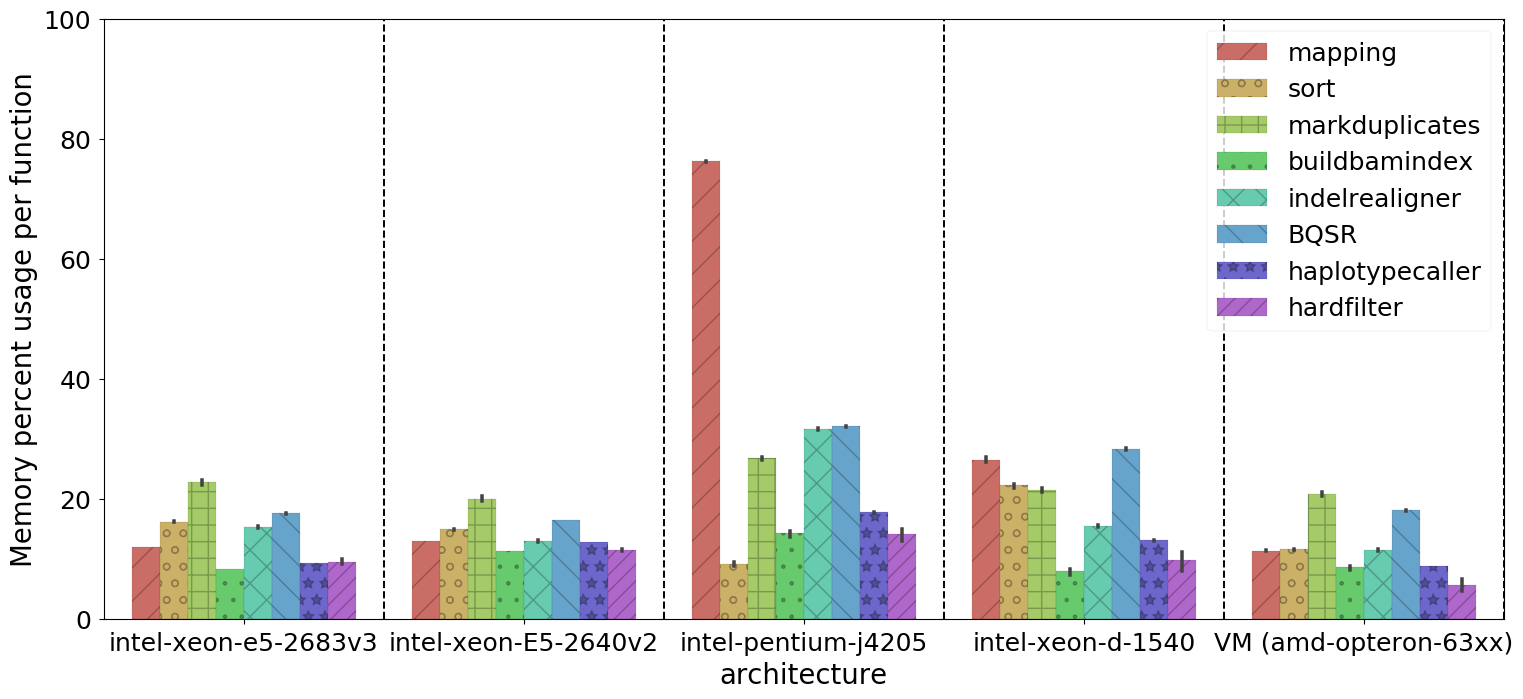
\includegraphics[width=\linewidth]{memory_per_function.png}
\caption{Memory used for each step of the pipeline. Due to the GATK memory allocation strategy, all steps use a baseline amount of memory proportional to the available memory. Smaller nodes, like the low power ones, require more memory as the baseline allocated memory is not sufficient to perform the calculation.}
\label{fig:memory-per-step}
\end{figure*}

\begin{figure*}[t!]
\centering
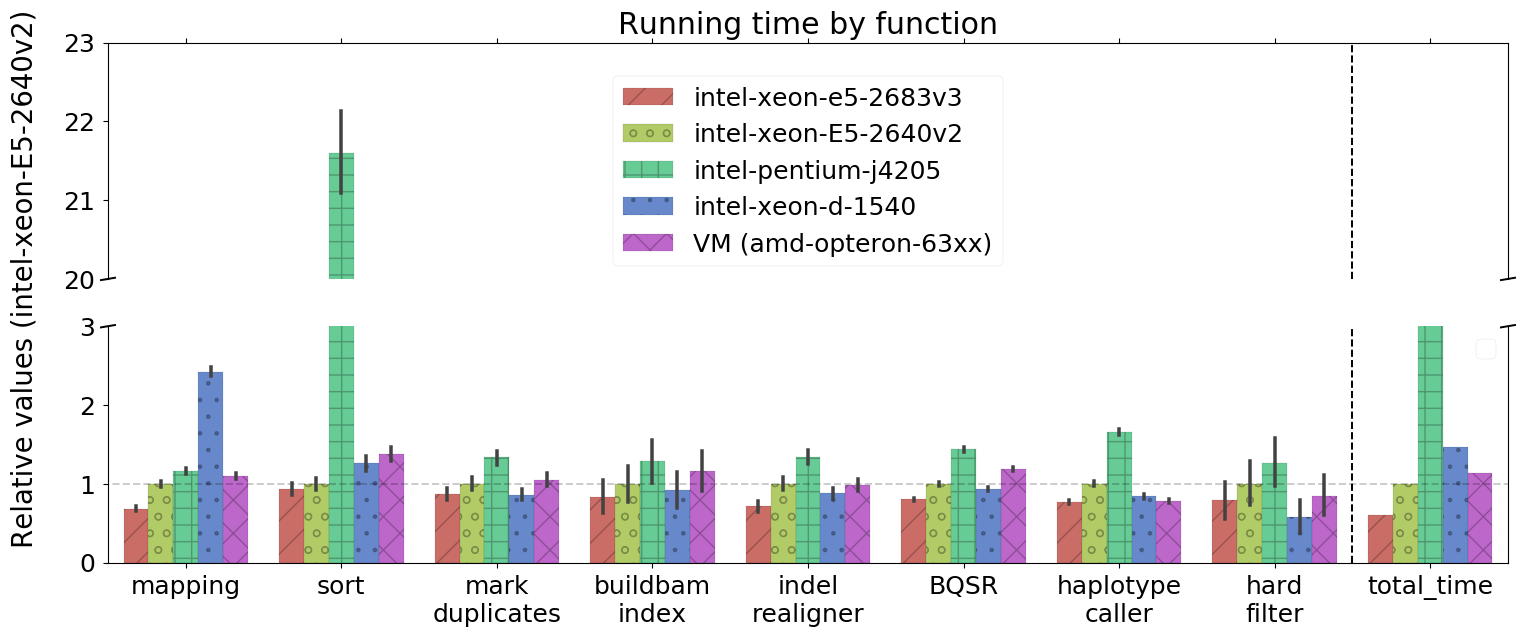
\includegraphics[width=\linewidth]{time_performances.png}
\caption{Time elapsed per step of the pipeline, and total elapsed time. In the sorting step, Pentium J is 20 times slower than the reference, probably due to the limited cache size.}
\label{fig:performance-per-step}
\end{figure*}

\begin{figure*}[t!]
\centering
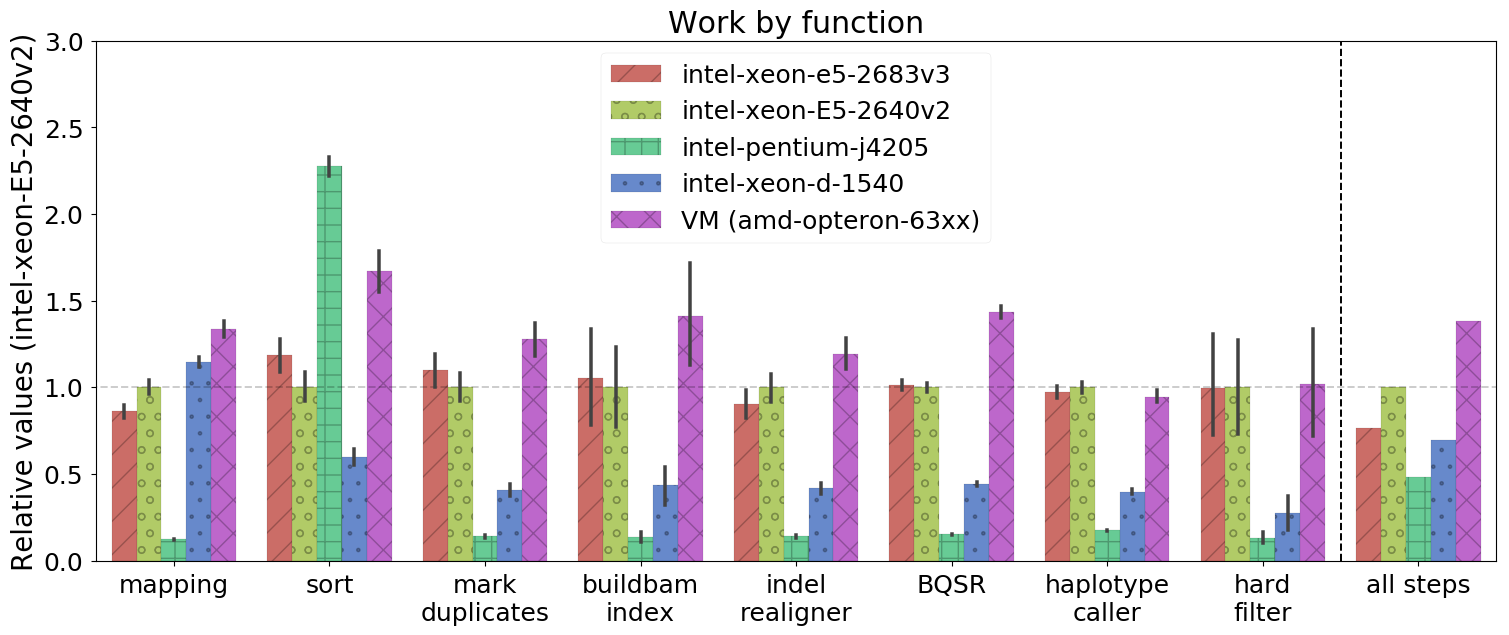
\includegraphics[width=\linewidth]{energy_and_cost.png}
\caption{Energy consumption per pipeline step and on the whole pipeline.
Energy consumption is estimated as the time taken by the step, multiplied by the number of cores used in the step and the power consumption per core (TDP divided by the available cores).
}
\label{fig:energy-per-step}
\end{figure*}




\section*{Conclusions}\addcontentsline{toc}{section}{Conclusions}
\markboth{Appendix F}{Conclusions}

Bioinformatics pipelines are one of the most important uses of biomedical big data and, at the same time, one of the hardest to optimize, both for their extreme requisites and the constant change of the specification, both in input-output data format and program API.

This makes the task of pipeline optimization a daunting one, especially for the final target of the results; physicians and biologists could lack the technical expertise (and time) required to optimize each new version of the various softwares of the pipelines.
Moreover, in a verified pipeline updating the software included without a long and detailed cross-validation with the previous one is often considered a bad practice: this means that often these pipelines are running with under-performing versions of each software.

Clinical use of these pipelines is growing, in particular with the rise of the concept of \quotes{personalized medicine}, where the therapy plan is designed on the specific genotype and phenotype of the individual patient rather than on the characteristic of the overall population.
This would increase the precision of the therapy and thus increase its efficacy, while cutting considerably the trial and error process required to identify promising target of therapy.
This requires the pipelines to be evaluated in real time, for multiple subjects at the same time (and potentially with multiple samples per subject).
To perform this task no single node is powerful enough, and thus it is necessary to use clusters.
This brings the need to evaluate which is the most cost and time efficient node that can be employed.

In the cost assessment there are several factors that need to be considered aside of the initial setup cost, namely cost for running the server and opportunity cost for obsolescence.
Scaled on medium sized facilities, such the one that could be required for a hospital, this cost could quickly overcome the setup cost.
This cost does also include not only the direct power consumption of the nodes, but also the required power for air conditioning to maintain them in the working temperature range.
Opportunity costs are more complex, but do represent the loss of possibility of using the most advanced technologies due to the cost of the individual node of the cluster.
Higher end nodes require a significant investment, and thus can not be replaced often.

With this perspective in mind, we surmise that energy efficient nodes present an interesting opportunity for the implementation of these pipelines.
As shown in this work, these nodes have a low cost per subject, paired with a low setup cost.
This makes them an interesting alternative to traditional nodes as a workhorse node for a cluster, as a greater number of cores can be bought and maintained for the same cost.

Given the high variability of the performances in the various steps, in particular with the sorting and mapping steps, it might be more efficient to employ a hybrid environment, where few high power nodes are used for specific tasks, while the bulk of the computation is done by the energy efficient nodes.
This is true even for those steps that can be massively parallelized, such as the mapping, as they benefit mainly from a high number of processors rather than few powerful ones.
In this work we focused only on CPUs computation, but another possibility could be an hybrid-parallelization approach in which the use of a single GPU accelerator can improve the parallelization of the slower steps.
Each pipeline work-flow requires its own analyses and tuning to reach the best performances and the right parallelization strategy based on the use which it is intended but a low energy node approach is emerging as a good alternative to the more expensive and common solutions.


\end{document}